%************************************************

\chapter{The turbulent gas structure in the centers of \ngc253 and the Milky Way}
\chaptermark{turbulent gas structure in galaxy centers}
\label{chapter: dendro}

%************************************************

\begin{papernote}
This chapter including appendix~\ref{appendix: dendro} comprises the article of the same title submitted the to Astrophysical Journal. The submitted paper has been reformatted to match the style of this thesis.
\end{papernote}


\begin{paperabstract}
We compare the molecular cloud properties in the starbursting center of \ngc253 and the Milky Way Galactic Center (GC) on scales of $\sim1$\,pc to several hundred pc by using resolution-, area- and noise-matched datasets.
Using dendrograms, we retrieve the hierarchical structure of the molecular interstellar medium in these galaxies from matched observations in \co10 and \co32.
We find that the size (R) -- line width ($\sigma$) relations in \ngc253 and the GC are similar in slope but \ngc253 has a significant offset towards larger line widths by factors of $\sim2-3.5$. The size--line width relation in \co32 is steep ($\sigma \propto R^{0.65\pm0.01}$ in \ngc253, $\sigma \propto R^{0.71\pm0.03}$ in the GC) but consistent with previous estimates in other molecular tracers. In \co10, the relations are steeper at $\sigma \propto R^{0.82\pm0.02}$ in \ngc253 and $\sigma \propto R^{0.84\pm0.09}$ in the GC.
The other structural properties of \ngc253 and the GC are very similar, including the size--luminosity relations as well as column density, volume density and mass probability density functions.
The size--line width coefficient ($\sigma^2/R$) dependency on column density $N$ shows that the increased line widths in \ngc253 originate in low column density gas ($N \LESSSIM 3 \times 10^{22}$\,\sqcm). 
In \ngc253, this analysis further implies a high external pressure ($P_\mathrm{ext} \sim 10^{7-7.5}$\,K\,\pcm3) and a significant amount of unbound (non-self-gravitating) molecular gas that is characterized by high velocity dispersion.
The unbound gas most likely corresponds to the known molecular outflows and potential diffuse molecular gas.
The excess kinetic energy of the unbound molecular gas in \ngc253 relative to the GC is most plausibly supplied by the starburst in the former as we show through estimation of the involved kinetic energies.
\end{paperabstract}


%%%%%%%%%%%%%%%%%%%%%%%%%%%%%%%%%%%%%%%%%%%%%%%%%%%%%%%%%%%%%%%%%%%%%%%%%%%%%%%%%%%%%%%%%%%%%%%%%%%%

\section{Introduction} \label{dendro: section: introduction}

The centers of spiral galaxies are special places in the galactic environment as their physical properties differ in many ways from the disk and halo. Even visible by the naked eye in nearby galaxies, stellar surface brightness is significantly higher in galaxy centers than in the disk. 
In strongly barred galaxies, the bar helps drive gas to the galaxy center \citep[e.g.][]{2019A&A...623A..79C}. This results in the formation of ring-like structures that are often connected to the outer galaxy by dust lanes and gas streams \citep[e.g.][]{2001AJ....121..225B,2017MNRAS.471.4027B,2017MNRAS.470.3819B,2005A&A...429..141K,2013A&A...555L...4C,2011A&A...529A..45V}. 
As all massive galaxies are thought to host a supermassive black hole (SMBH) in their centers \citep{2013ARA&A..51..511K}, the picture is even more complex, especially if the SMBH is actively accreting, i.e. it is visible as an active galactic nucleus (AGN) and affecting its surroundings through AGN feedback. 
In addition, close to the bottom of the galactic gravitational potential (on $10^2$\,pc scales), the rotation curve transitions from its typically flat shape to solid body\linebreak[4] rotation -- this changes the dynamical forces acting on the gas \citep[e.g.][]{2017MNRAS.466.1213K}. All these properties (and more) create a unique gravitational, dynamical and highly complex environment for the star formation life cycle.

As a result of these conditions, the gas contents of galactic centers are typically characterised by more extreme properties than the surrounding disk: higher densities, higher temperatures, and higher velocity dispersion and turbulence \citep[e.g.][]{Morris:1996db,2000ApJ...536..357M,2001ApJ...562..348O,2012MNRAS.425..720S,2013PASJ...65..118S,2016A&A...586A..50G,2017ApJ...850...77K,2019MNRAS.483.4291C,2019ApJ...871..170M}. According to star formation prescriptions that focus on density \citep{2013MNRAS.429..987L,Kennicutt:1998id,2005ApJ...630..250K,Krumholz:2012ja,Lada:2012it,2010ApJ...724..687L} an elevated star formation rate (SFR) would consequently be expected which is not always found.

Galactic centers and (nuclear) starbursts are often referred to as analogs for high-z star forming galaxies at the peak of the cosmic star formations history \citep[e.g.][]{2013MNRAS.435.2598K}. Upon closer inspection, however, these proposed high-z analogs can differ significantly in properties of the ISM, stellar content, star formation process and feedback \citep[e.g.][]{2017MNRAS.471.2311L,2019ApJ...872..146J}.

Studies of star forming regions within the Milky Way allow for very high spatial resolution and show that it is necessary to resolve individual clouds at pc-scales to correctly capture the physical processes that are relevant for the star formation process. 
With the newest and upcoming generations of radio telescopes it is now feasible to resolve the necessary scales in nearby galaxies such as \ngc253.

For the first time, we conduct a matched comparison of the properties of the turbulent molecular ISM at parsec scale resolution in the nearby universe and interpret the results in the context of the star formation process.
In this work, we focus on the Milky Way's more quiescent Galactic Center (GC) and the center of \ngc253 which harbors a nuclear starburst.

This paper is structured as follows: In Section~\ref{dendro: section: data}, we describe the datasets of \ngc253 and the GC. The methodological approach of the dendrogram technique and how to construct size--line width relations is laid out in Section~\ref{dendro: section: structural analysis}. We show the results (Section~\ref{dendro: section: results}), discuss them in Section~\ref{dendro: section: discussion} and summarise our work in Section~\ref{dendro: section: summary}. The appendix~\ref{appendix: dendro: structure definition} lists technical details and presents checks of the used methods.

\subsection{The Galactic Center}

At a distance of only $\sim8.2$\,kpc, the GC is the nearest galactic center and can be observed at unrivaled resolution.
The GC (central $\sim 1$\,kpc) hosts a significant fraction of order 10\% of the entire molecular gas mass of the Milky Way with $\sim 6-8 \times 10^7$\,\Msun of molecular gas in the Central Molecular Zone \citep{1998ApJS..118..455O,Morris:1996db,2007A&A...467..611F}.
Compared to the high mass of dense molecular gas available for star formation, it shows a low SFR ($\sim 0.1$\Msunyr) and SFR density despite hosting many of the galaxy's most massive and dense molecular clouds \citep[e.g.][]{2013MNRAS.429..987L,2017MNRAS.469.2263B}.
As a result, the star formation efficiency of the dense gas is also very low compared to the Galactic disk \citep[e.g.][]{2013MNRAS.429..987L}.
This discrepancy has been attributed to cloud stabilization by turbulent pressure and a quiescent phase of episodic \citep[e.g.][]{2015MNRAS.453..739K,2017MNRAS.466.1213K} or stochastic \citep[e.g.][]{2019MNRAS.484.1213S} gas processes and star formation.
Increasing evidences for winds and outflows from the GC hint towards more active star formation (or AGN activity) in the past \citep[e.g.][]{2019arXiv191106864L,2019MNRAS.482.4813S}.

Throughout this paper, we adopt the recent precise distance measurement of 8.178\,kpc for the GC \citep{2019A&A...625L..10G} for which 10\,pc correspond to 4.2\arcmin.
We refer to Sgr~A* at $l, b = 359.94422947^\circ, -0.04615714^\circ$ as the ``central position'' of the GC \citep{2011AJ....142...35P}. For the systemic velocity we use 0\,\kms.


\subsection{\ngc253 and its starbursting center}

\ngc253 is one of the nearest starburst systems (SFR $\sim 2$\,\Msunyr in the central $\sim 500$\,pc) at a distance of 3.5\,Mpc \citep{Rekola:2005ha} and hosts a collection of dense, massive molecular clumps associated with star formation \citep[e.g.][]{Sakamoto:2011et,2017ApJ...849...81A}. \citet{2018ApJ...869..126L} showed that these clumps contain 14 forming super star clusters (SSCs). With these properties, \ngc253 is considered one of the prototypical bar-fed nuclear starburst galaxies.
A star formation driven galactic wind emerges from the central $\sim 200$\,pc of \ngc253 that has been characterized in H$\alpha$, X-ray, as well as neutral and molecular gas emission \citep[e.g.][]{Sharp:2010jl,Turner:1985iy,Sturm:2011jb,Strickland:2000wd,Strickland:2002kp, Westmoquette:2011bp,2000ApJS..129..493H,2013Natur.499..450B,2017ApJ...835..265W,2019ApJ...881...43K,2006ApJ...636..685S}. 
Studies of the molecular gas phase in \ngc253 demonstrated that its central starburst occurs within a molecular gas reservoir of $\sim 3-4 \times 10^8$\,\Msun \citep{1996A&A...305..421M,Leroy:2015ds,2018ApJ...860...23P,2019ApJ...881...43K} and refueled by gas accretion along the bar \citep{2004ApJ...611..835P}.
The inclination of $i = 78^\circ$ makes \ngc253 an ideal target to compare to the Milky Way GC at $i \sim 90^\circ$ because the geometric corrections are relatively small ($\sin [78^\circ] = 0.98 \sim \sin [90^\circ]$).

For the remainder of this paper, we refer to the central $\sim 800$\,pc of \ngc253 where the starburst is located simply as \ngc253.
The ``central position'' of \ngc253 denotes the kinematic center at $\alpha, \delta = 00^h47^m33.134^s, -25^\circ17^m19.68^s$ as identified in \citet{MullerSanchez:2010dr} at a systemic velocity of 250\,\kms.
At a distance of 3.5\,Mpc \citep{Rekola:2005ha}, 10\,pc correspond to 0.59\arcsec.


%%%%%%%%%%%%%%%%%%%%%%%%%%%%%%%%%%%%%%%%%%%%%%%%%%%%%%%%%%%%%%%%%%%%%%%%%%%%%%%%%%%%%%%%%%%%%%%%%%%%
% DATA
%%%%%%%%%%%%%%%%%%%%%%%%%%%%%%%%%%%%%%%%%%%%%%%%%%%%%%%%%%%%%%%%%%%%%%%%%%%%%%%%%%%%%%%%%%%%%%%%%%%%

\section{Data}
\label{dendro: section: data}

\begin{table}
    \centering
    \footnotesize
    \begin{threeparttable}
        \caption[Details of the datasets used in the dendrogram analysis]{Details of the datasets used in this analysis.
        \label{dendro: table: 1}}
        
        \begin{tabular}{llccccll}
            \toprule
            set & source & line & \multicolumn{2}{c}{resolution} & noise$^b$ & reference & ALMA ID\\
	        &&& spectral & physical$^a$ &      &&\\
	        &&& [\kms]   & [pc]         & [mK] &\\
            \midrule
{\parbox[t]{2mm}{\multirow{2}{*}{\rotatebox[origin=c]{90}{low}}}} & GC & \co10 & 5.0 & 32.0 & 38 & \textsc{COGAL} \citet{2001ApJ...547..792D} &\\
& \ngc253 & \co10 & 5.0 & 32.0 & 38 & \citet{2013Natur.499..450B} & 2011.1.00172.S\\
\rule{0pt}{4ex} 
{\parbox[t]{2mm}{\multirow{2}{*}{\rotatebox[origin=c]{90}{high}}}} & GC     & \co32 & 2.5 & \phantom{3}3.0 & 115 &  Eden et al., (in prep) &\\
& \ngc253 & \co32 & 2.5 & \phantom{3}3.0 & 115 & \citet{2019ApJ...881...43K} & 2015.1.00274.S\\
            \bottomrule
        \end{tabular}
	    \begin{tablenotes}
	        \item[a] FHWM of the circular beam.
            \item[b] Root mean square noise in line-free channels after matching the noise by adding beam-correlated Gaussian noise to the GC data.
        \end{tablenotes}
    \end{threeparttable}
\end{table}

Our goal is to measure if and how the size--line width relation differs between \ngc253 and the Galactic Center. For a robust comparison, we need to match the data by comparing the same tracers at the same resolution. CO line emission is the standard tracer molecule for the diffuse to moderately dense molecular medium. We use \co10 for a low resolution comparison and \co32 for a high resolution comparison.

For \ngc253, we use the ALMA \co10 observations from \citet{2013Natur.499..450B}, \citet{Leroy:2015ds} and \citet{2015ApJ...801...63M} and the ALMA \co32 from \citet{2019ApJ...881...43K}. We refer to those papers for details of the data reduction and imaging. 

The \textsc{COGAL} survey imaged the entire Galactic plane in \co10 including the GC using the 1.2\,m Millimeter-Wave Telescope at the CfA \citep{2001ApJ...547..792D}. The \textsc{CHIMPS2} project (Eden et al., in prep.) extends the \textsc{CHIMPS} \co32 Galactic plane survey \citep{2016MNRAS.456.2885R} at the James Clerk Maxwell Telescope into the inner Galactic plane and the Central Molecular Zone building upon the data reduction recipe of COHRS \citep[CO high-resolution survey of the Galactic plane;][]{2013ApJS..209....8D}.
It must be noted that the \co10 COGAL survey undersamples the Galactic plane at $\sim 1$ beam spacing which was then interpolated to obtain a filled map whereas the other datasets (CHIMPS2, \ngc253 ALMA) are fully sampled.

Since we aim to carefully compare two environments in two galaxy centers, we match the data as closely as possible to eliminate potential artifacts. Specifically, we match spatial and spectral resolution, pixel scale, orientation with respect to the galactic plane, field of view (FoV) and noise.

\begin{enumerate}[noitemsep,topsep=0pt]
\item[(1)] The images are smoothed to circular beams with the highest possible common resolution (32\,pc for \co10 and 3.0\,pc for \co32).
\item[(2)] The images are then reprojected onto a common pixel grid aligned with galactic longitude and latitude. Pixel scales are 6.4\,pc and 0.6\,pc for \co10 and \co32, respectively (factor 5 oversampling).
\item[(3)] The spectral resolution is matched to 5.0\,\kms for \co10 and 2.5\,\kms for \co32 and reprojected on the same grid with respect to systemic velocity. The images cover radial velocities from $-250$\,\kms to $+250$\,\kms for both sources and CO lines.
\item[(4)] The field of view is restricted to the overlap between the images so that we study the same amount of area in each galaxy. Centered on the respective galactic center, the FoVs are 1500\,pc by 750\,pc for the wider FoV in \co10 and 800\,pc by 400\,pc in \co32. 
\item[(5)] After these steps, the noise in the datasets varies by a factor of $\sim 2$ between the \ngc253 and the GC datasets. To keep the analysis consistent between the two galaxies, we add additional beam-correlated\footnote{Random noise that has been convolved with a Gaussian beam and scaled to the appropriate level.} Gaussian noise to both GC images to match them to the higher noise of the \ngc253 observations. For the CHIMPS2 data, the noise varies spatially across the map and we add noise as needed to achieve a uniform noise level. The final rms noise is 38\,mK in a 5.0\,\kms channel in \co10 and 115\,mK in a 2.5\,\kms channel in \co32.
\end{enumerate}

The final image parameters are given in Table~\ref{dendro: table: 1}.
The beam filling factors of the final images should be very similar in each of the \co10 and \co32 images because we match the physical resolution and there is no indication of significantly different cloud sizes.


%%%%%%%%%%%%%%%%%%%%%%%%%%%%%%%%%%%%%%%%%%%%%%%%%%%%%%%%%%%%%%%%%%%%%%%%%%%%%%%%%%%%%%%%%%%%%%%%%%%%
% ANALYSIS
%%%%%%%%%%%%%%%%%%%%%%%%%%%%%%%%%%%%%%%%%%%%%%%%%%%%%%%%%%%%%%%%%%%%%%%%%%%%%%%%%%%%%%%%%%%%%%%%%%%%

\section{Structural analysis}
\label{dendro: section: structural analysis}

In this work, we compare the molecular gas properties in \ngc253 and the GC through standard scaling relations that are briefly explained in the following.

\subsection{The size--line width relation}

The first of the three ``Larson laws'' relates the projected size $R$ of a cloud to the line width $\sigma$ measured in the same cloud \citep{Larson:1981jma}. It is commonly expressed as a power law of form
\begin{equation}
    \sigma = a R^{b}
    \label{equation: size-line width}
\end{equation}
with normalisation $a$ and exponent $b$. \citet{Larson:1981jma} originally found a relation of $\sigma = 1.10 R^{0.38}$ for $\sigma$ in \kms and $R$ in pc using primarily the optically thin tracer $^{13}$CO for Milky Way disk clouds. Other authors have expanded this method to further tracers and environments and found exponents of $0.2 - 0.6$ \citep[e.g.][]{1987ApJ...319..730S,Bolatto:2008iv,Heyer:2009ii,2012MNRAS.425..720S}. 
Idealized theoretical arguments imply an exponent $b=0.5$ for bound clouds in which velocity dispersion (turbulence) balances self-gravity according to compressible turbulence \citep[e.g.][]{2007ARA&A..45..565M}.


\subsection{The size -- mass (luminosity) relation}

The size--mass relation is a direct consequence of the ``third Larson law'' $n \propto R^q$ that relates volume density $n$ and size $R$. Integrating this relation over the volume of a cloud results in a relation of mass $M$ and size.
A better observational parametrization of this relation is the size--luminosity relation.
\begin{equation}
    L = c R^{d}
    \label{equation: size-luminosity}
\end{equation}
Using luminosity instead of mass has the benefit of being independent of uncertain and potentially varying light-to-mass conversion factors. For a constant mass-to-luminosity ratio (e.g. a fixed $\alpha_\mathrm{CO}$ conversion factor) both relation are equivalent modulo the conversion factor.

\citet{Larson:1981jm}'s original work implies $d=1.9$ while modern studies in the Milky Way typically find values of $d=2.0$ for extinction-derived mass \citep[e.g.][ for local clouds without significant projection effects]{2010A&A...519L...7L} and $d=2.2-2.4$ for CO based estimates \citep[e.g.][]{2010ApJ...723..492R,2017ApJ...834...57M}.
\citet{2019MNRAS.490.2648B} recently argued that the value $d\GTR 2$ is the result of line-of-sight superposition for an intrinsic exponent of $d=2$ in Galactic CO surveys. Observational artifacts may thus influence observed size--mass (luminosity) relations.


%%%%%%%%%%%%%%%%%%%%%%%%%%%%%%%%%%%%%%%%%%%%%%%%%%%%%%%%%%%%%%%%%%%%%%%%%%%%%%%%%%%%%%%%%%%%%%%%%%%%

\subsection{Dendrogram analysis}
\label{dendro: section: dendrogram}

To study the turbulent gas properties through the size--line width and size--luminosity relations, structures need to be defined in a consistent way for which sizes and line widths can be measured. Ideally, one would like to recover the 3D volume of a molecular cloud as the entity to analyze, yet we do not have knowledge of the actual 3D structure of the target but only the projected view. However, in (sub-)millimeter spectral line observations, a spectral coordinate is virtually always measured and thus velocity can help in separating 2D projections. 
Recently, \citet{2019arXiv191007692L} test several common clump detection algorithms and found so-called dendrograms to be among the best methods due to high accuracy and detection completeness. Dendrograms have also become a standard technique to analyse the molecular ISM over the past years which allows for a more direct comparison to the literature.

The \astrodendro package that we use in this work, captures the hierarchical structure of molecular clouds as a tree of nested structures called ``branches'' and ``leaves''. A detailed description of these so-called dendrograms is given in the literature \citep[e.g.][]{2008ApJ...679.1338R,Goodman:2009dp,2012MNRAS.425..720S} or on the \astrodendro homepage\footnote{\url{dendrograms.readthedocs.io}}. Each structure (``branch'') is embedded within a larger structure down to the ``trunk'' and contains one or more smaller structures within, up to the ``leaves''.
Note that this method is a parametrization of the hierarchical structure of the input data and a given structure does not necessarily correspond to a (giant) molecular cloud. Especially the small leaves on top of nested branches are not independent molecular clouds but substructure in the data that could be described as ``cloudlets'' or ``cores'' within a cloud.

The identification of structures is based on several thresholds that define a volume contiguous across spatial and spectral coordinates in a position-position-velocity (PPV) data cube. A structure can thus be understood as a closed isocontour in PPV space. 
To calculate the structures, a lower cut-off on intensity (minimum intensity) is placed to only consider pixels with significant emission avoiding noise. 
Starting from local maxima, the algorithm searches for underlying larger structures to which the difference in intensity needs to be higher than a second threshold (minimum delta between structures).
A third threshold defines the minimum volume a structure can have, which removes unresolved structures. In this process, a tree of hierarchical structures is built bottom-up.

We consider only emission with SNR $\GTR 5$ with the dataset-dependent rms noise (cf. Table~\ref{dendro: table: 1}). The minimum difference in intensity between nested structures is set to the rms noise. 
We require the minimum volume per structure to be three times the spatial resolution element (synthesized beam) times velocity channel width.


%%%%%%%%%%%%%%%%%%%%%%%%%%%%%%%%%%%%%%%%%%%%%%%%%%%%%%%%%%%%%%%%%%%%%%%%%%%%%%%%%%%%%%%%%%%%%%%%%%%%

\begin{figure}[t]
    \centering
    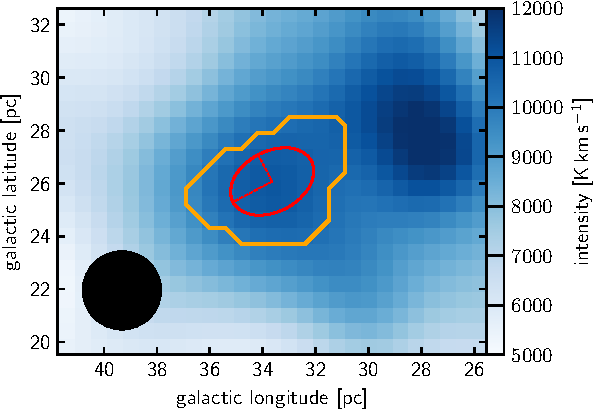
\includegraphics[width=0.6\linewidth]{images/chapters/papers/dendro/dendro_fig1}
    \caption[Example how \astrodendro assigns sizes to structures]{Example how \astrodendro assigns sizes to structures. The figure shows a random structure (\#4822) in the \co32 dataset of \ngc253 which contains a local emission peak. The total extent of the structure (orange) and the corresponding intensity-weighted second moment ellipse (red) are plotted on top of the total integrated intensity (0$^\mathrm{th}$ moment) \co32 map (blue). Dashed lines indicate the semi-major and semi-minor axes whereof the mean defines the size of the structure, here 1.20\,pc. The beam of 3\,pc FWHM is shown in the bottom left corner.
    Note that the background image shows all data to provide context whereas the size ellipse is calculated for the particular structure within the orange line.
    In this special case of a small structure, the algorithm described in Section~\ref{dendro: section: dendrogram size} assigns a size smaller than the beam to the structure. Nevertheless, the structure is resolved. Despite this effect, the \astrodendro definition of structure size has multiple advantages (cf. Appendix~\ref{appendix: dendro: size definition} for details).
    \label{dendro: figure: 1}}
\end{figure}

We define four properties from the dendrogram structures for our analysis:

\subsubsection{Size}
\label{dendro: section: dendrogram size}

We define the size $R$ of a structure as the arithmetic mean of the semi-major and semi-minor axis extent in position-position (PP) plane. The major and minor axes are defined by the projection of the PPV structure onto the PP plane, computed from the intensity weighted second moment in direction of greatest elongation in the PP plane. This definition is implemented in \astrodendro as the \texttt{radius} quantity.
In Appendix~\ref{appendix: dendro: size definition}, we explore the effect of different definitions of $R$ and conclude that it does not influence the derived size--line width relation considerably.

Note that \astrodendro parametrizes size as a semi axis (instead of full axis) which allows for resolved structures apparently smaller than the spatial resolution (given as FWHM). Furthermore, this definition incorporates intensity weighting and will thus assign sizes smaller than half the resolution to structures approaching to the resolution limit. The exact value depends on the distribution of emission within the structure. The chosen minimum PPV volume threshold in dendrogram ensures that a structure is resolved and derived sizes smaller than the resolution do \emph{not} mean that a structure is unresolved.
Figure~\ref{dendro: figure: 1} shows an example of a small but resolved structure in \co32 in \ngc253. The size inferred by the algorithm above is 1.20\,pc and thus less than half the FWHM beam size.
Note that we do not deconvolve the beam from the structure size and report the \astrodendro definition of size.


\subsubsection{Line width}
\label{dendro: section: dendrogram line width}

The velocity dispersion of a structure is defined as the intensity-weighted second moment (intensity-weighted velocity dispersion) over the pixels belonging to the structure as is implemented in \astrodendro as the \texttt{v\_rms} quantity.
Other definitions of line width can influence derived relations and can introduce artifacts as we test in Appendix~\ref{appendix: dendro: line width definition}.
We do not deconvolve the channel width from the obtained linewidths.
Note that projection effects can broaden the linewidth. Two clouds towards the same spatial position but separated along the line-of-sight may blend in velocity space and \astrodendro identifies them as a single structure. The linewidth of such a structure is broadened by the velocity difference between the constituent clouds which in turn depends on galactic dynamics, e.g. galactic rotation. 
Since the line width is derived on a per-pixel basis, bulk motions across the spatial extent of a structure do not influence the line width.


\subsubsection{Luminosity}
\label{dendro: section: luminosity}
We calculate the luminosity of each structure as the area integrated intensity $L = \int I \mathrm{d}A$ which translates to $L = \sum_i I_i \times A_\mathrm{pix}$ for discrete data with pixel area $A_\mathrm{pix}$. The integrated intensity $\sum_i I_i$ is reported directly by \astrodendro.


\subsubsection{Column density}
\label{dendro: section: dendrogram column density}

Following the typical approach in the literature, we define the column density $N$ of a structure as the number of H$_2$ atoms per effective area $A_\mathrm{eff}$.
The number of atoms per pixel $i$ is the product of CO-to-H$_2$ conversion factor $X_\mathrm{CO}$, flux $F_i$ and pixel area $A_\mathrm{pix}$, corrected for the line ratio in the case of \co32.
The effective area of a structure is defined as the luminosity--weighted ellipse area $A_\mathrm{eff} = n_\mathrm{pix}^\mathrm{eff} A_\mathrm{pix}$ with the effective number of pixels $n_\mathrm{pix}$. 
The area of a pixel $A_\mathrm{pix}$ cancels out and $N$ becomes:
\begin{equation}
    N_\mathrm{H_2} = \frac{\sum_i \frac{X_\mathrm{CO}}{r} F_i}{n_\mathrm{pix}^\mathrm{eff}}
    \label{equation: column density}
\end{equation}
We adopt standard \co10 conversion factors as listed in Table~\ref{dendro: table: conversion factors}.

To translate this to a \co32 conversion factor, we use the mean line ratio $r_{31} = I_{3-2}\,I_{1-0} ^{-1} = 0.67$.
The line ratios $r_{31}$ measured from the data convolved to the same resolution within the overlap area are $0.63$ in \ngc253 and $0.68$ in the GC. However, these measurements are poorly sampled due to the large \co10 beam (32\,pc) compared to the small overlap area defined by the \co32 field-of-view ($800\,\mathrm{pc} \times 400$\,pc). Also the line ratios outside the \co32 field-of-view cannot be measured from the data.
We therefore adopt a common line ratio of $r_{31}=0.67$ and note that other choices linearly scale the obtained column density.


\begin{table}
    \centering
    \begin{threeparttable}
        \caption[Gas mass conversion factors]{Conversion factors used in this analysis.
        \label{dendro: table: conversion factors}}
        
        \begin{tabular}{lccl}
            \toprule
            source & $X_\mathrm{CO}$ & $\alpha_\mathrm{CO}$ & Ref. \\
            & $\left[\frac{\mathrm{cm}^{-2}}{\mathrm{K\,km\,s}^{-1}}\right]$ & $\left[\frac{\mathrm{M}_\odot}{\mathrm{K\,km\,s}^{-1}\,\mathrm{pc}^2}\right]$ & \\[2mm]
            \midrule
\ngc253  & $0.5\times10^{20}$ & $1.1$ & L15, B13\\
GC      & $1.0\times10^{20}$ & $2.2$ & M99, Y03, B13\\
            \bottomrule
        \end{tabular}
        \tablenote{These conversion factors apply for \co10. We assume line ratios $r_{31} = I_{3-2}\,I_{1-0} ^{-1} = 0.67$ to correct higher excitation state of the \co32 lines.}
        \\
        \tablereference{L15 \citep{Leroy:2015ds}, B13 \citep{2013ARA&A..51..207B}, M99 \citep{1999A&A...341..256M}, Y03 \citep{2003ApJ...588..771Y}}
    \end{threeparttable}
\end{table}


\subsubsection{Mass}
\label{dendro: section: dendrogram mass}

The mass $M_\mathrm{struct}$ of a structure follows from the H$_2$ column density $N_\mathrm{struct}$  and the area $A_\mathrm{struct}$ as
\begin{equation}
    M_\mathrm{struct} = 1.36 \times 2\,\mathrm{u} \times N_\mathrm{struct} A_\mathrm{struct}
    \label{equation: mass}
\end{equation}
with the mass 2\,u (atomic unit $\mathrm{u}=1.66\times10^{-27}$\,kg) for a hydrogen molecule and the factor 1.36 corrects for the relative contribution of helium.
Note that this mass estimate traces the luminous mass (in contrast to the virial mass).


\subsubsection{Virial state}
\label{dendro: section: dendrogram virial state}

Molecular clouds are often assumed to be structures roughly in virial equilibrium \citep[e.g.][]{1987ApJ...319..730S} for which the deviation is expressed as the virial parameter $\avir = 2K / U$ where $K$ is the kinetic energy and $U$ the gravitational potential. Following \citet{2018ApJ...860..172S} for idealized spherical clouds, it is possible to relate its line width $\sigma$, virial parameter \avir, size $R$ and average column density $N$ (Eq.~\ref{equation: column density}) according to
\begin{equation}
    N = \frac{5}{f \avir G \pi} \frac{\sigma^2}{R},
\end{equation}
where $G$ is the gravitational constant, the factor $f = (1-\gamma/3)/(1-2\gamma/5)$ accounts for the internal cloud structure with a radial density profile $\rho(r) \propto r^{-\gamma}$. For $\gamma = 1$, thus $f = 10/9$.
This idealized case is certainly not correct for real molecular clouds but the deviation from an isolated self-gravitating cloud can reveal insight into its dynamic state and the contribution of other forces such as external pressure or magnetic support.

The effect of external pressure on the size--line width coefficient $\sigma^2/R$ has been worked out by \citet{2011MNRAS.416..710F} as
\begin{equation}
    \frac{\sigma^2}{R} = \frac{1}{3} \left( \pi \Gamma G \Sigma + \frac{4P_e}{\Sigma}\right)
\end{equation}
where $G$ is the gravitational constant, $\Sigma$ the mass column density and $P_e$ the external pressure. The form factor $\Gamma$ is $3/5$ for a spherical cloud of constant density or 0.73 for an isothermal spherical cloud of critical mass (used in the following). We include the contribution of helium to the mass and derive the mass column density $\Sigma = 1.36 \times 2\,\mathrm{u} \times N$ from the number column density $N$.


%%%%%%%%%%%%%%%%%%%%%%%%%%%%%%%%%%%%%%%%%%%%%%%%%%%%%%%%%%%%%%%%%%%%%%%%%%%%%%%%%%%%%%%%%%%%%%%%%%%%

\subsection{Binned analysis}
\label{dendro: section: binning}

The dendrogram analysis yields a very high number of structures, e.g. $\GTR 12,000$ individual structures in the \co32 data of \ngc253. As we are interested in the statistical properties of the clouds, we bin the structures in size bins of 0.1\,dex. Binning gives us the quantity of interest: the typical line width or luminosity at a fixed size scale, e.g. the scale of a molecular cloud ($\sim 10$\,pc) or a GMC ($\sim 100$\,pc). For each size bin, we report the median line width and the $16^{th}$ to $84^{th}$ percentile range as a measure of the line width spread. We exclude bins with less than three entries to get meaningful binned data. We further exclude the dendrogram trunks.
We explored various bin sizes and found 0.1\,dex to provide a good compromise between the number of bins and elements per bin.
For exploring the virial state of the gas in Section~\ref{dendro: section: virial state}, we apply the same binning approach with a bin size of 0.25\,dex. Since these data span a larger dynamical range, a larger bin size is optimal.

The minimum-volume-of-a-structure threshold imposes a diagonal cutoff in size-line width space.
We exclude the affected size interval from the analysis as listed in Table~\ref{dendro: table:  size limits}.
This effectively also excludes the smallest structures that are affected by beam convolution and channel convolution.
The corrections for beam convolution are $\LESS 25$\% even at the lower limits of sizes considered (Table~\ref{dendro: table:  size limits}). Given this we make no corrections.
As will be shown in Section~\ref{dendro: section: results}, the GC data is found at lower line width than the \ngc253 data, so the minimum-volume threshold affects the distribution starting at larger sizes in the GC. As a result the minimum recoverable size scale differs across sources although the datasets are at identical resolution.

We also cannot recover the largest size scales because they are dominated by galactic motions as explained in Section~\ref{dendro: section: dendrogram line width}. We find that the transition towards that regime is unexpectedly sharp and it is thus possible to remove affected structures based on a cut on size. Table~\ref{dendro: table:  size limits} shows the upper limits. They differ between sources but also depend on the (spatial and spectral) resolution of the data since coarser resolution creates more blending.

\begin{table}
    \centering
    \begin{threeparttable}
        \caption[Limits on recoverable structure sizes]{Limits on recoverable structure sizes.
        \label{dendro: table:  size limits}}
        
        \begin{tabular}{llcc}
            \toprule
            source & line & $R_\mathrm{min}$ & $R_\mathrm{max}$\\
                  &      & (1)              & (2)\\
            \midrule
\ngc253 & \co10 & 0.55 & 18\\
GC     & \co10 & 0.90 & 20\\
\ngc253 & \co32 & 6.0 & 60\\
GC     & \co32 & 8.5 & 68\\
            \bottomrule
        \end{tabular}
	    \tablenonote{(1) Completeness limit imposed by the minimum-volume-of-a-structure threshold.\\
        (2) Limit beyond which large scale dynamics (e.g. galactic rotation) dominate structure properties.
        }
    \end{threeparttable}
\end{table}


%%%%%%%%%%%%%%%%%%%%%%%%%%%%%%%%%%%%%%%%%%%%%%%%%%%%%%%%%%%%%%%%%%%%%%%%%%%%%%%%%%%%%%%%%%%%%%%%%%%%

\subsection{Fitting}
\label{dendro: section: fitting}

The size-binned size--line width and size--luminosity relations follow a power law and can be fitted with a weighted least squares minimization in logarithmic space. We report the square root of the diagonals of the covariance matrix as the errors for normalization $a$ and exponent $b$ as defined in Equation~\ref{equation: size-line width}. 
These statistical errors are often small as will be shown in the following Section~\ref{dendro: section: results} and systematic errors are non-negligible.

The normalization $a$ corresponds to the typical line width at a size scale of 1\,pc. Given the coarser resolution of the data, the line width at a scale of 10\,pc is a more meaningful measure of typical line width and we report this quantity as \sigmaten.
Similarly, for the size--luminosity relation we report \Lten as the typical luminosity of a 10\,pc sized structure instead of the normalization $c$.


%%%%%%%%%%%%%%%%%%%%%%%%%%%%%%%%%%%%%%%%%%%%%%%%%%%%%%%%%%%%%%%%%%%%%%%%%%%%%%%%%%%%%%%%%%%%%%%%%%%%
% RESULTS
%%%%%%%%%%%%%%%%%%%%%%%%%%%%%%%%%%%%%%%%%%%%%%%%%%%%%%%%%%%%%%%%%%%%%%%%%%%%%%%%%%%%%%%%%%%%%%%%%%%%

\section{Results}
\label{dendro: section: results}

In the following, we present the derived size--line width and size--luminosity relations as well as an analysis of the size--line width coefficient. For each of those analyses individually, we first present data on the GC and \ngc253 followed by a comparison.


%%%%%%%%%%%%%%%%%%%%%%%%%%%%%%%%%%%%%%%%%%%%%%%%%%%%%%%%%%%%%%%%%%%%%%%%%%%%%%%%%%%%%%%%%%%%%%%%%%%%

\subsection{Size -- line width relation}
\label{dendro: section: size line width}

Figure~\ref{dendro: figure: 2} presents the binned size--line width relation obtained as described in Section~\ref{dendro: section: structural analysis}. With the high resolution \co32 data, we are able to cover the size range down to $\LESS 1$\,pc whereas the lower resolution \co10 covers the larger scales up to $\sim 90$\,pc.
Details of the dendrogram statistics and power law fits to the size--line width relation are listed in Table~\ref{dendro: table: 2}.

\begin{figure}
    \centering
    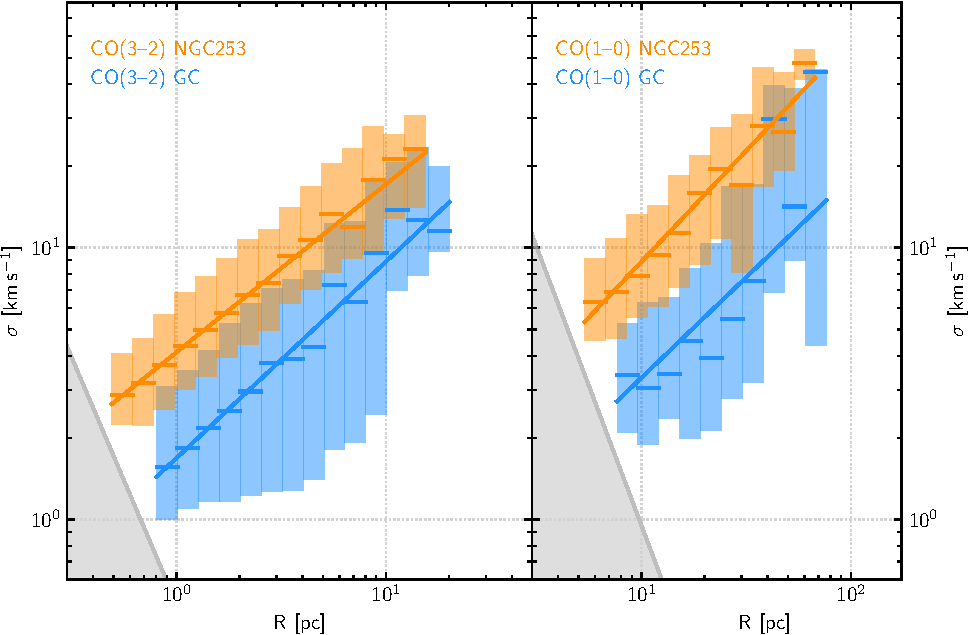
\includegraphics[width=\textwidth]{images/chapters/papers/dendro/dendro_fig2}
    \caption[Size--line width relation]{Binned size--line width relation for \co32 (\emph{left}) and \co10 (\emph{right}) in \ngc253 (orange) and the GC (blue). Horizontal lines indicate the median of the distribution of line widths (colored bars) in each bin. The values of the power law fits (solid lines) are given in Table~\ref{dendro: table: 2}. Grey, shaded areas indicate the minimum volume limit that ensures structures are significantly detected.
    The size--line width relation in \ngc253 is significantly offset towards larger line widths from the relation in the GC for both tracers.
    \label{dendro: figure: 2}}
\end{figure}


\begin{table}
    \centering
    \footnotesize
    \begin{threeparttable}
        \caption[Dendrogram statistics and fit results for size--line width and size--mass relations]{Dendrogram statistics and fit results for power law fits to the binned size--linewidth and size--luminosity relations shown in Figure~\ref{dendro: figure: 1} and \ref{dendro: figure: 3}.
        \label{dendro: table: 2}}
        
        \begin{tabular}{lcrrrcccc}
            \toprule
            source & line & \multicolumn{3}{c}{dendrogram structures} & \multicolumn{2}{c}{size--linewidth} & \multicolumn{2}{c}{size--luminosity}\\
            && total & branches & leaves & $b$ & \sigmaten & $d$ & log $\Lten$ \\
            &&&&& (1) & (2) & (3) & (4)\\
            \midrule
\ngc253 & CO(1--0) &   991 &  466 &  520 & $0.82\pm0.02$ & $ 8.9\pm0.2$ & $2.92\pm0.07$ & $4.27\pm0.11$ \\
GC     & CO(1--0) &   324 &  158 &  165 & $0.74\pm0.04$ & $ 3.3\pm0.4$ & $3.25\pm0.13$ & $4.34\pm0.20$ \\
\ngc253 & CO(3--2) & 12414 & 5145 & 7024 & $0.62\pm0.01$ & $17.1\pm0.1$ & $2.89\pm0.02$ & $5.44\pm0.03$ \\
GC     & CO(3--2) & 10235 & 4563 & 5570 & $0.72\pm0.03$ & $ 8.9\pm0.2$ & $2.69\pm0.02$ & $4.96\pm0.02$ \\
            \bottomrule
        \end{tabular}
	    \tablenonote{(1) Exponent $b$ of the power law fit to the size--linewidth relation according to Equation~\ref{equation: size-line width}.\\
        (2) Characteristic linewidth at 10\,pc according to the power law fit to the size--linewidth relation (Equation~\ref{equation: size-line width}) in \kms.\\
        (3) Exponent $d$ of the power law fit to the size--luminosity relation according to Equation~\ref{equation: size-luminosity}.\\
        (4) Characteristic luminosity at 10\,pc according to Equation~\ref{equation: size-luminosity} in $\log \mathrm{M}_\odot$.
        }
    \end{threeparttable}
\end{table}


%%%%%%%%%%%%%%%%%%%%%%%%%%%%%%%%%%%%%%%%%%%%%%%%%%%%%%%%%%%%%%%%%%%%%%%%%%%%%%%%%%%%%%%%%%%%%%%%%%%%

\subsubsection{Galactic Center}
\label{dendro: section: size line width: GC}

For the GC \co32, the binned data (Figure~\ref{dendro: figure: 2}, left) closely follow a power law. In \co10, the binned data (Figure~\ref{dendro: figure: 2}, right) scatter and do not follow a power law as closely as the \co32 does. The \co10 relation is less certain due to the low number of 324 recovered structures.
The power law fit according to Eq.~\ref{equation: size-line width} yields exponents of $b=0.72 \pm 0.03$ in \co32 and $b=0.74 \pm 0.04$ in \co10. 
The typical line width at 10\,pc derived from the fit is $\sigmaten = 8.9 \pm 0.2$\,\kms in \co32 and $\sigmaten = 3.3\pm0.9$\,\kms in \co10.

%%%%%%%%%%%%%%%%%%%%%%%%%%%%%%%%%%%%%%%%%%%%%%%%%%%%%%%%%%%%%%%%%%%%%%%%%%%%%%%%%%%%%%%%%%%%%%%%%%%%

\subsubsection{\ngc253}
\label{dendro: section: size line width: ngc253}

In \ngc253, the binned \co32 data (Figure~\ref{dendro: figure: 2}, left) almost perfectly follows a power law over more than one order of magnitude. In \co10, the statistical basis is weaker and the binned data (Figure~\ref{dendro: figure: 2}, right) shows a higher level of scatter than \co32 but the data still closely follows a power law relation.
A fit according to Eq.~\ref{equation: size-line width} results in exponents of $b=0.62 \pm 0.01$ in \co32 and $b=0.82 \pm 0.02$ in \co10. 
The fit yields typical line widths at 10\,pc of $\sigmaten = 17.1 \pm 0.1$\,\kms in \co32 and $\sigmaten = 8.9 \pm 0.2$\,\kms in \co10.

%%%%%%%%%%%%%%%%%%%%%%%%%%%%%%%%%%%%%%%%%%%%%%%%%%%%%%%%%%%%%%%%%%%%%%%%%%%%%%%%%%%%%%%%%%%%%%%%%%%%

\subsubsection{Comparison of the size -- line width relations}
\label{dendro: section: size line width: comparison}

The size--line width relations in the GC and \ngc253 are significantly offset from each other at similar slopes. In both cases, \co10 and \co32, the GC size--line width relation is offset towards smaller line widths compared to \ngc253. The line widths are wider in \ngc253 by a factor $\sim 1.9$ and $\sim 2.7$ for \co32 and \co10, respectively. Parametrized as \sigmaten (cf. Section~\ref{dendro: section: fitting}), the GC shows consistently smaller line widths by 8.2\,\kms (\co32) and 5.6\,\kms (\co10). In both \co10 and \co32, the offset is roughly constant across size, i.e. the line width ratio between \ngc253 and the GC is constant.
As mentioned in Section~\ref{dendro: section: size line width: GC}, the lower number of structures potentially affects the power law fit to the \co10 GC data. However, even if so, Figure~\ref{dendro: figure: 2} (right) consistently shows significantly smaller line widths\footnote{This also applies to the unbinned data.} than in \ngc253.

It is also noteworthy that the GC shows a wider distribution of line widths than \ngc253 at a fixed size scale. This implies a greater variation of turbulent cloud properties in the GC and more uniform clouds in \ngc253.

When comparing the two CO lines in each galaxy center, the line widths at $8-16$\,pc scales do not match but the \co32 lines are wider. In \ngc253, this difference is $\sim 8$\,\kms (factor $\sim 1.9$) and $\sim 6$\,\kms (factor $\sim 2.7$) in the GC.
This is opposite to the expectation that \co10 should trace larger and more diffuse structures with greater turbulent motions and thus line widths.

The reason for the observation of lower line widths in \co10 is about equal parts the change in image resolution and tracer properties of the CO lines. As a test, we degrade the resolution of the \co32 data in \ngc253 losing the ability to probe size scales $\LESS 10$\,pc and redo the dendrogram analysis. Degrading the spatial (6.4\,pc to 32\,pc in ten steps to match the \co10 data) and spectral (2.5\,\kms to 5.0\,\kms) resolution causes a shift of the size--line width relation towards larger sizes (to the right-hand side in Figure~\ref{dendro: figure: 2}) approximately linear with resolution. At a fixed size scale, the measured line width is thus smaller with lower resolution data. Half of the observed line width mismatch is explained directly as a consequence of these resolution effects. 
The other half is related to the tracer properties of the CO lines and specifics of the dendrogram algorithm\footnote{A large structure can include multiple peaks (smaller substructures) along the line-of-sight. Due to excitation with $r_{31}\LESS 1$ the gas in between the peaks is fainter in \co32 than \co10. The linewidth derived as the intensity-weighted second moment is thus smaller for the \co10 structure. The same effect causes the linewidth to increase when decreasing the resolution as emission is spread out spatially. The impact of this effect on a given structure depends greatly on the specific configuration and excitation. Trunks as the largest structures are strongly affected but typically, the nested substructure splits rapidly (the dendrogram tree branch out quickly after the trunk level) and thus the effect quickly becomes negligible towards nested structures.}.
As we are interested in the comparison across environment (\ngc253 vs. GC), we will not discuss this effect further.


%%%%%%%%%%%%%%%%%%%%%%%%%%%%%%%%%%%%%%%%%%%%%%%%%%%%%%%%%%%%%%%%%%%%%%%%%%%%%%%%%%%%%%%%%%%%%%%%%%%%

\subsection{Size -- luminosity relation}
\label{dendro: section: size luminosity}

\begin{figure}
    \centering
    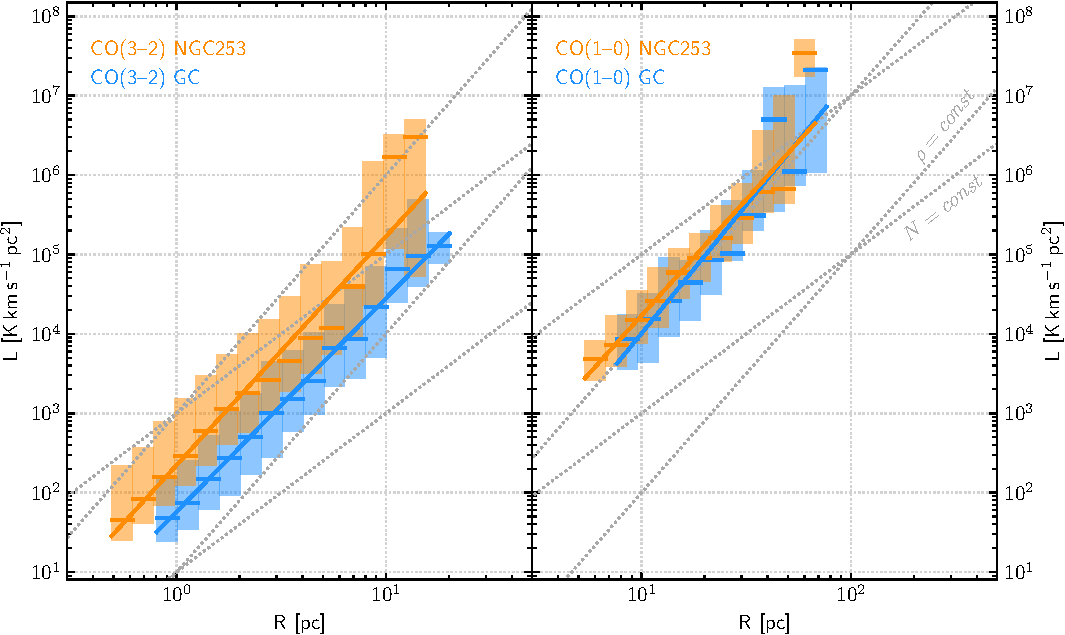
\includegraphics[width=\textwidth]{images/chapters/papers/dendro/dendro_fig3}
    \caption[Size--luminosity relation]{Relation between dendrogram structure size and luminosity for \co32 (\emph{left}) and \co10 (\emph{right}) in \ngc253 and the GC. Horizontal lines indicate the median of the distribution of luminosities (colored bars) in each bin. The values of the power law fits (solid lines) are given in Table~\ref{dendro: table: 2}.
    In each panel, two lines of constant surface density $N$ ($M \propto L \propto R^2$) and constant volume density $\rho$ ($M \propto L \propto R^3$) are shown for reference.
    }
    \label{dendro: figure: 3}
\end{figure}

Figure~\ref{dendro: figure: 3} shows the size--luminosity relation and Table~\ref{dendro: table: 2} lists the power law fit parameters according to Equation~\ref{equation: size-luminosity}.
In Appendix~\ref{appendix: dendro: size mass}, we also show the size--mass relation after applying the conversion factors listed in Table~\ref{dendro: table: conversion factors} to Figure~\ref{dendro: figure: 3}.


%%%%%%%%%%%%%%%%%%%%%%%%%%%%%%%%%%%%%%%%%%%%%%%%%%%%%%%%%%%%%%%%%%%%%%%%%%%%%%%%%%%%%%%%%%%%%%%%%%%%

\subsubsection{Galactic Center}
\label{dendro: section: size luminosity: GC}

The binned size--luminosity relations for \co10 and \co32 in the GC scale very close to power laws.
The fits yield power law exponents of $d=2.69 \pm 0.02$ in \co32 and $d=3.25 \pm 0.13$ in \co10.
The high slope in \co10 is influenced by the last bin ($R\sim80$\,pc). Without this bin, the slope is consistent with a more moderate $d=3$.
A power law exponent $\LESS 3$ in \co32 implies decreasing volume density for large size structures whereas the higher exponent $\GTR 3$ in \co10 indicates increasing volume density with size. Note, however, that the \co10 relation is less certain due to the low number of 324 recovered structures.

%%%%%%%%%%%%%%%%%%%%%%%%%%%%%%%%%%%%%%%%%%%%%%%%%%%%%%%%%%%%%%%%%%%%%%%%%%%%%%%%%%%%%%%%%%%%%%%%%%%%

\subsubsection{\ngc253}
\label{dendro: section: size luminosity: ngc253}

In \ngc253, the binned size--luminosity relations also scale nearly perfectly as power laws.
Although we remove the dendrogram trunks and large scale structures affected by galactic dynamics, the largest size scale bins in Figure~\ref{dendro: figure: 3} are still somewhat affected as can be seen by the sudden upturn of the relations. However, this only negligibly affects the power law fits which yield exponents of $d=2.89 \pm 0.02$ in \co32 and $d=2.92 \pm 0.07$ in \co10.
These exponents $d \sim 3$ imply approximately constant volume density independent of the structure size.

%%%%%%%%%%%%%%%%%%%%%%%%%%%%%%%%%%%%%%%%%%%%%%%%%%%%%%%%%%%%%%%%%%%%%%%%%%%%%%%%%%%%%%%%%%%%%%%%%%%%

\subsubsection{Comparison of the size -- luminosity relation}
\label{dendro: section: size luminosity: comparison}

Figure~\ref{dendro: figure: 3} shows that there is little difference in the size--luminosity relations between \ngc253 and the GC.
In \co10, the relations are almost identical within the scatter. The \co32 size--luminosity relations are offset by a factor $\sim 2-3$ with higher luminosities in \ngc253. 
Taken together this implies higher excitation in \ngc253.
Higher luminosities in \ngc253 than in the GC are expected since the former is known to be more massive and brighter.

The size--mass relations (Appendix~\ref{appendix: dendro: size mass}) that follow from Figure~\ref{dendro: figure: 3} after applying the conversion factors listed in Table~\ref{dendro: table: conversion factors} eliminate the luminosity offset in \co32 between \ngc253 and the GC. In \co10, the sources remain very close in their size--mass relation.

Reflecting the data, the power law fits are similar as well. In \co32, the exponents are identical within the errors while for \co10 the exponents differ by $\sim10$\%. Within the distribution of the data (indicated by the bars in Figure~\ref{dendro: figure: 3}), exponents deviating systematically by up to 20\% from the best fit are plausible.
In \co10, the power law normalisations \Lten of GC and \ngc253 are consistent but significantly smaller than for \co32.
As for the size--line width relation, the two CO tracers do not match at the overlapping size scale of $8-16$\,pc. This is caused by the differing resolutions and tracer properties (cf. Section~\ref{dendro: section: size line width: comparison}).

In addition to the similar size--luminosity relations, we further conclude that there is no significant difference in the density and mass structures between \ngc253 and the GC by comparing the column density, volume density and mass probability distribution functions (PDFs). Appendix~\ref{appendix: dendro: mass density structure} shows these PDFs and discusses their properties.


%%%%%%%%%%%%%%%%%%%%%%%%%%%%%%%%%%%%%%%%%%%%%%%%%%%%%%%%%%%%%%%%%%%%%%%%%%%%%%%%%%%%%%%%%%%%%%%%%%%%

\subsection{Virial state of the molecular gas}
\label{dendro: section: virial state}

In order to explore the origin of the differing size--line width relations in \ngc253 and the GC, we now examine the virial state (Section~\ref{dendro: section: dendrogram virial state}) of the obtained structures. This analysis assumes that the luminous mass (Section~\ref{dendro: section: dendrogram mass}) derived from CO is a good mass estimate and explores the dynamical state of the structures implied by the size--line width relations (Section~\ref{dendro: section: size line width}).

\begin{figure}[t]
    \centering
    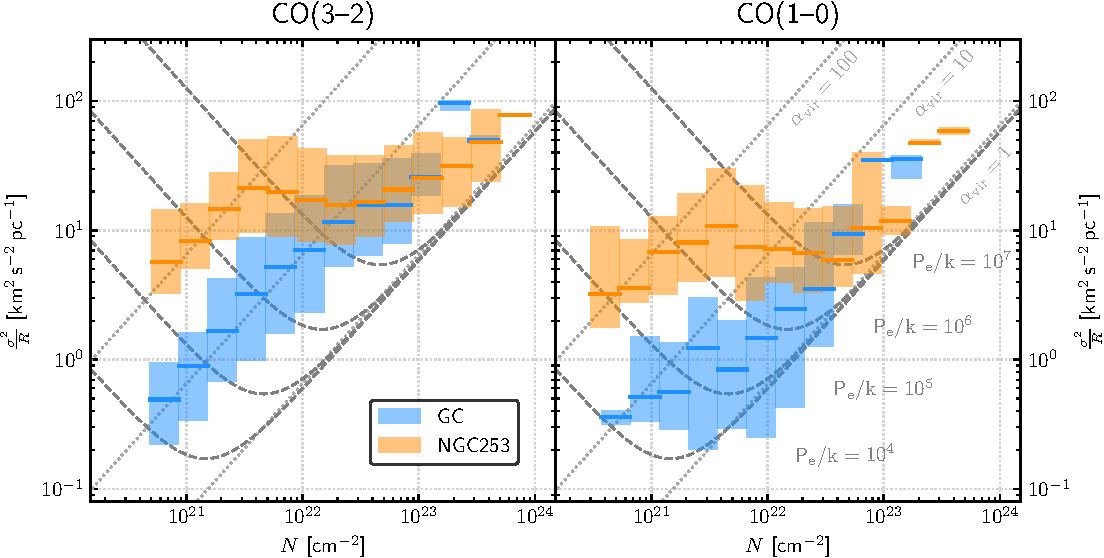
\includegraphics[width=\textwidth]{images/chapters/papers/dendro/dendro_fig4}
    \caption[Size--line width coefficient vs. column density relation]{Size--line width coefficient as a function of column density in \ngc253 and the GC under the assumption that luminous (CO detected) mass traces virial (gravitational) mass. Diagonal lines indicate lines of constant virial parameter under the assumption of spherical clouds (cf. Section~\ref{dendro: section: virial state}). V-shaped lines represent lines of constant external pressure on an idealized spherical cloud (cf. Section~\ref{dendro: section: virial state}). Horizontal lines indicate the median of the distribution of $\Sigma^2/R$ (colored bars) in each bin. \emph{left}: low resolution \co10; \emph{right}: high resolution \co32. 
    Note that the derived column density should be considered a lower limit (cf. Section~\ref{dendro: section: physical implications}). A different choice of conversion factors shifts the obtained relations along the x-axis but does not influence the slope.
    Due to the similar geometry and gas distribution in \ngc253 and the GC, a relative comparison is still possible even if the absolute values must be interpreted with care. The strongly enhanced $\sigma^2/R$ at column densities $N \LESSSIM 3 \times 10^{22}$\,\sqcm implies that the low column density molecular gas in \ngc253 is gravitationally unbound which is not the case in the GC. Appendix~\ref{appendix: dendro: virial state separated} shows this plot separated in size bins to address the degeneracy between $\sigma$ and $R$ in the size--line width coefficient.
    }
    \label{dendro: figure: 4}
\end{figure}

Figure~\ref{dendro: figure: 4} shows the $\sigma^2/R$ (size--line width coefficient) versus column density $N$ relation. For reference, Figure~\ref{dendro: figure: 4} shows lines of constant virial parameter at $\avir = 1, 10, 100$ and lines of constant external pressure at $P_e = 10^4, 10^5, 10^6, 10^7$\,K\,\pcm3.

For the interpretation of Figure~\ref{dendro: figure: 4}, it must be kept in mind what a dendrogram structure is (cf. Section~\ref{dendro: section: structural analysis}): a data parametrization that does not necessarily correspond to the simplistic idea of a cloud as an independent entity.
Care must thus be taken when trying to interpret Figure~\ref{dendro: figure: 4} as the virial state of clouds of a certain size.
Especially on scales of a few parsecs, this figure shows the dependence of $\sigma^2/R$ on $N$ for substructures within larger objects rather than ``clouds''. On such small size scales other contributions to the line width like internal motions and pressure must be taken into account. Hence, a comparison with the theoretical lines for virial parameter and external pressure can not be interpreted to yield absolute values but indicate qualitative and relative differences.

Figure~\ref{dendro: figure: 4} shows all data regardless of size or line width. The size--line width coefficient $\sigma^2/R$ is thus degenerate between size and line width. Separating Figure~\ref{dendro: figure: 4} by size or line width does not change the picture, though, as we show in Appendix~\ref{appendix: dendro: virial state separated}. The relations seen in Figure~\ref{dendro: figure: 4} also hold when separating by structure size (Figure~\ref{dendro: figure: D}).


%%%%%%%%%%%%%%%%%%%%%%%%%%%%%%%%%%%%%%%%%%%%%%%%%%%%%%%%%%%%%%%%%%%%%%%%%%%%%%%%%%%%%%%%%%%%%%%%%%%%

\subsubsection{Galactic Center}
\label{dendro: section: size virial state: GC}

Figure~\ref{dendro: figure: 4} (right) shows that for \co10, $\sigma^2/R$ scales with column density approximately as a power law with unity exponent, i.e. at constant virial parameter.
The \co32 data (Figure~\ref{dendro: figure: 4}, left) also follows a power law scaling with column density but at an overall higher virial parameter ($\alpha \sim 10$) than \co10 ($\alpha \sim3-10$).

%%%%%%%%%%%%%%%%%%%%%%%%%%%%%%%%%%%%%%%%%%%%%%%%%%%%%%%%%%%%%%%%%%%%%%%%%%%%%%%%%%%%%%%%%%%%%%%%%%%%

\subsubsection{\ngc253}
\label{dendro: section: size virial state: ngc253}

For \ngc253, both \co10 and \co32 show a more complicated relation between $\sigma^2/R$ and column density.
Towards high column densities of $N \GTRSIM 3 \times 10^{22}$\,\sqcm and low column densities of $N \LESSSIM 3 \times 10^{21}$\,\sqcm the data suggests a power law scaling roughly consistent with a constant virial parameter.
At high column densities, the virial parameters are therefore significantly lower ($\alpha \sim 2-10$) than in the low column density regime ($\alpha \sim 100$).
In the intermediate range of $3 \times 10^{22}\,\mathrm{cm}^{-2} \GTRSIM N \GTRSIM 3 \times 10^{21}$\,\sqcm, the size--line width coefficient is approximately constant and the medians even temporarily decreases with increasing column density. The hint towards a local dip in $\sigma^2/R$ for \co10 falls on the minimum of the constant pressure line with $P_e \sim 10^7$\,K\,\pcm3 and for \co32 the local dip corresponds to $P_e \sim 10^{7.5}$\,K\,\pcm3. This implies high external pressures in the center of \ngc253.


%%%%%%%%%%%%%%%%%%%%%%%%%%%%%%%%%%%%%%%%%%%%%%%%%%%%%%%%%%%%%%%%%%%%%%%%%%%%%%%%%%%%%%%%%%%%%%%%%%%%

\subsubsection{Comparison of the virial state}
\label{dendro: section: size virial state: comparison}

\ngc253 and the GC behave very differently in $\sigma^2/R$--$N$ space. 
In both \co10 and \co32, the Galactic Center structures scale with decreasing $\sigma^2/R$ towards lower column density at roughly constant virial parameter.
For the \ngc253 structures, however, a potential power law scaling is broken at intermediate column densities. This causes the relations in \ngc253 to deviate from the GC relations at $N \LESSSIM 3 \times 10^{22}$\,\sqcm. At $N \GTRSIM 3 \times 10^{22}$\,\sqcm no significant difference between \ngc253 and the GC is apparent and structures in both sources are found at low virial parameters of a few.


%%%%%%%%%%%%%%%%%%%%%%%%%%%%%%%%%%%%%%%%%%%%%%%%%%%%%%%%%%%%%%%%%%%%%%%%%%%%%%%%%%%%%%%%%%%%%%%%%%%%
% DISCUSSION
%%%%%%%%%%%%%%%%%%%%%%%%%%%%%%%%%%%%%%%%%%%%%%%%%%%%%%%%%%%%%%%%%%%%%%%%%%%%%%%%%%%%%%%%%%%%%%%%%%%%

\section{Discussion}
\label{dendro: section: discussion}

%%%%%%%%%%%%%%%%%%%%%%%%%%%%%%%%%%%%%%%%%%%%%%%%%%%%%%%%%%%%%%%%%%%%%%%%%%%%%%%%%%%%%%%%%%%%%%%%%%%%

\subsection{Comparison to the literature}
\label{dendro: section: literature}

We now compare our results to the vast body of literature work on scaling relations in various environments within and outside of the Milky Way.

There are different effects that either increase or reduce the observed exponents of the scaling relations depending on specific details of the used cloud identification algorithm and the unknown exact geometry along the line-of-sight towards the source.
The simulations by \citet{2010ApJ...712.1049S} show that the intrinsic size--linewidth exponents can be even steeper than the exponent retrieved from position-position-velocity (PPV) data. This happens because the PPV analysis can split up large clouds into several smaller structures due to intrinsic velocity gradients along the line-of-sight.
On the other hand, the intrinsic exponent may be more shallow than an observed exponent due to line-of-sight contamination by low levels of unrelated emission at similar velocities \citep{2019MNRAS.490.2648B}. Such contamination more often affects farther away and larger clouds and thus steepens the exponent.
This is the same effect as we observe for the largest structures (Section~\ref{dendro: section: dendrogram line width}).

Hence, differences in the source orientation and tracer properties may significantly influence the obtained size--linewidth and size--luminosity exponents and comparisons across the literature have to be considered carefully.


%%%%%%%%%%%%%%%%%%%%%%%%%%%%%%%%%%%%%%%%%%%%%%%%%%%%%%%%%%%%%%%%%%%%%%%%%%%%%%%%%%%%%%%%%%%%%%%%%%%%

\subsubsection{Size--line width relation}
\label{dendro: section: literature: size line width}

\begin{figure}[t]
    \centering
    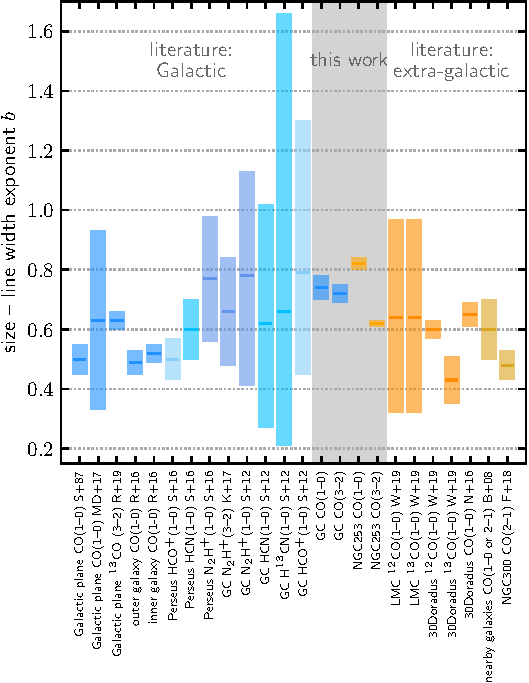
\includegraphics[width=0.6\linewidth]{images/chapters/papers/dendro/dendro_fig5}
    \caption[Literature comparison: size--line width exponent]{The size--line width exponent $b$ as in $\sigma \propto R^b$ derived in this work compared to Galactic and extra-galactic literature. Molecular tracers are colorcoded in shades of blue for Galactic measurements and shades of orange for extra-galactic measurements. The shown studies vary strongly in the size scale over which the exponent $b$ was derived from $\LESS 1$\,pc to $\sim 200$\,pc. See Section~\ref{dendro: section: literature: size line width} for details. The abbreviated references refer to (ordered left to right): S+87 \citep{1987ApJ...319..730S}, MD+17 \citep{2017ApJ...834...57M}, R+19 \citep{2019A&A...632A..58R}, R+16 \citep{2016ApJ...822...52R}, S+16 \citep{Storm:2016cl}, K+17 \citep{2017A&A...603A..89K}, S+12 \citep{2012MNRAS.425..720S}, W+19 \citep{2019ApJ...885...50W}, N+16 \citep{2016ApJ...831...32N}, B+08 \citep{Bolatto:2008iv} and F+18 \citep{2018ApJ...857...19F}.}
    \label{dendro: figure: 5}
\end{figure}

Figure~\ref{dendro: figure: 5} shows an overview of the literature including our new measurements that we will discuss in the following.
We find $b=0.65 \pm 0.01$ (\co32, \ngc253), $b=0.72 \pm 0.03$ (\co32, GC) as well as $b=0.82 \pm 0.02$ (\co10, \ngc253) and $b=0.74\pm0.04$ (\co10, GC).
In the GC, \citet{2012MNRAS.425..720S} found $b=0.62-0.79$ for dense gas tracers (N$_2$H$^+$, HCN, H$^{13}$CN, HCO$^+$) where $b$ spans Bayesian 95\% highest density intervals (95\%HDI) of $0.2-1.6$ (equivalent to $2\sigma$ errors in the case of Gaussian distributions). Their error interval is thus approximately twice as large compared to the usual $1\sigma$ intervals. Further observations by \citet{2017A&A...603A..89K} confirm the steep relation in the GC $b=0.66\pm0.18$ using N$_2$H$^+$. Both of these studies cover size scales up to $\sim 40$\,pc \citep{2012MNRAS.425..720S} and $\sim 8$\,pc \citep{2017A&A...603A..89K} and are thus consistent with our results in both the GC and \ngc253.
\citet{2017ApJ...834...57M} found $b=0.63 \pm 0.30$ for $\GTR 8000$ $^{12}$CO(1--0) clouds in the Galactic plane \citep[using the][survey]{2001ApJ...547..792D} on size scales $\LESS 1$\,pc to $\GTRSIM 200$\,pc which is confirmed by \citet{2019A&A...632A..58R} with $b=0.63\pm0.03$ for $^{13}$\co32. Using the same \co10 data, \citep{2016ApJ...822...52R} did a dendrogram analysis for the inner and outer galaxy separately resulting in $b=0.52\pm0.03$ (inner galaxy) and $b=0.49\pm0.04$ (outer galaxy). They also find a significantly higher normalization in the inner galaxy (corresponding to $\sigmaten = 1.65\pm0.20$\,\kms and $\sigmaten = 1.17\pm0.19$\,\kms for inner and outer galaxy, respectively) indicating pressure confinement of clouds in the inner galaxy. This is lower than our result of $\sigmaten = 3.3\pm0.4$\,\kms for \co10 in the GC implying that the GC is a region of broader line widths within the inner galaxy.
Star formation regions in the Milky Way outside the GC typically exhibit $b\sim 0.5-0.7$ \citep[e.g.][]{1987ApJ...319..730S,Storm:2016cl} across a wide range of covered size scales ($\LESS 0.1$\,pc to $\LESSSIM 100$\,pc in these studies).

In the LMC, \citet{2019ApJ...885...50W} find a combined $b=0.64$ in $^{12}$CO(1--0) and $b=0.59$ in $^{13}$CO(1--0) with significant scatter across the six mapped regions ($b=0.32-0.97$ and $b=0.36-1.00$ for $^{12}$CO and $^{13}$CO, respectively). They find $b=0.60\pm0.03$ ($^{12}$CO) and $b=0.43\pm0.08$ ($^{13}$CO) for the high-mass star forming region 30~Doradus similar to e.g. \citet{2016ApJ...831...32N} with $b=0.65\pm0.04$ ($^{12}$\co21). These studies in the LMC also cover small size scales of $3-15$\,pc \citep{2019ApJ...885...50W} and $0.15-5$\,pc \citep{2016ApJ...831...32N}. Across the disks of nearby galaxies comparable values have been obtained on GMC scales at $\GTRSIM 30-50$\,pc resolution (e.g. $b=0.60\pm0.60$ \citealt{Bolatto:2008iv}; $b=0.48\pm0.05$, NGC300, \citealt{2018ApJ...857...19F}).

\citet{Wong:2017hx} note a striking deviation in the size--line width normalization of factor of $\sim 5$ between the quiescent Planck cold cloud and the star formation region 30~Doradus. Consistent across $^{12}$CO and $^{13}$CO, they conclude that this difference is unlikely to be caused by optical depth. The enhanced line width in the star formation region relative to a quiescent region is qualitatively consistent with our observation of the factor $1.9-2.7$ enhancement in \ngc253 relative to the GC.

Our new measurements of the size--line width exponent in \ngc253 are therefore consistent with previous studies in the Galactic Center and star forming galaxies. The measurements in the GC are also compatible with previous measurements in the same region, albeit with different tracers.


%%%%%%%%%%%%%%%%%%%%%%%%%%%%%%%%%%%%%%%%%%%%%%%%%%%%%%%%%%%%%%%%%%%%%%%%%%%%%%%%%%%%%%%%%%%%%%%%%%%%

\subsubsection{Size -- luminosity (mass) relation}
\label{dendro: section: literature: size mass}

\begin{figure}[t]
    \centering
    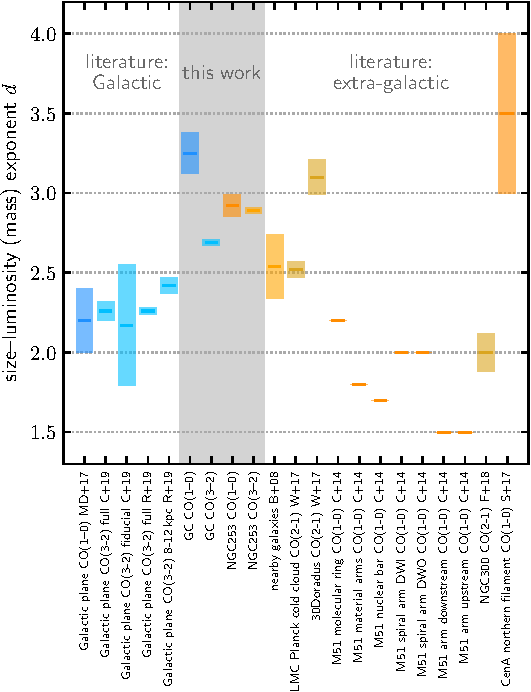
\includegraphics[width=0.6\linewidth]{images/chapters/papers/dendro/dendro_fig6}
    \caption[Literature comparison: size--luminosity exponent]{The size--luminosity (mass) exponent $d$ as in $L \propto R^d$ (or $m \propto R^d$) derived in this work compared to Galactic and extra-galactic literature. Molecular tracers are colorcoded in shades of blue for Galactic measurements and shades of orange for extra-galactic measurements. The shown studies vary strongly in the size scale over which the exponent $d$ was derived from $\LESS 1$\,pc to $\sim 200$\,pc. See Section~\ref{dendro: section: literature: size mass} for details. The abbreviated references refer to (ordered left to right): MD+17 \citep{2017ApJ...834...57M}, C+19 \citep{2019MNRAS.483.4291C}, R+19 \citep{2019A&A...632A..58R}, B+08 \citep{Bolatto:2008iv}, W+17 \citep{Wong:2017hx}, C+14 \citep[cf. definitions of the regions within M51]{2014ApJ...784....3C}, F+18 \citep{2018ApJ...857...19F}, S+17 \citep{2017A&A...608A..98S}.}
    \label{dendro: figure: 6}
\end{figure}

We derive steep size--luminosity relations with power law exponents $d\sim3$. In the GC, \co10 yields the steepest exponent at $d=3.25\pm0.13$ while the exponent derived from \co32 is more shallow at $d=2.69\pm0.02$. The results for \ngc253 are consistent at $d=2.92\pm0.07$ (\co10) and $d=2.89\pm0.02$ (\co32).

Figure~\ref{dendro: figure: 6} gives an overview of the size--mass exponent found in this study and in the literature which is discussed in the following.
\citet{2017ApJ...834...57M}, using the \citet{2001ApJ...547..792D} Galactic plane CO data, obtained a power law exponent $d=2.2 \pm 0.2$ for $\GTR 8000$ clouds in the Galactic plane.
In the Milky Way first quadrant (using the COHRS \co32 data, \citealt{2013ApJS..209....8D}), \citet{2019MNRAS.483.4291C} find $d=2.26\pm0.06$ in their sample of $\GTR 85000$ disk clouds and $d=2.17\pm0.38$ in the subsample with good distance estimates.
Very similar results are found by \citet{2019A&A...632A..58R} using the CHIMPS \co32 data with $d=2.26\pm0.02$ (full sample) and $d=2.42\pm0.05$ (distance $8-12$\,kpc) for disk clouds.
No size--luminosity or size--mass relations across a collection of clouds are reported in the literature for the GC yet\footnote{\citet{2017A&A...603A..90K} report exponents of $d\sim1$ and $d\sim1.7$ within six selected clouds in the GC. Their derivation of the exponent from two observations of different resolution strongly differs from data segmentation approaches like dendrograms.}

Steeper exponents $d \GTRSIM 2.5$ are commonly encountered in nearby extra-galactic studies on GMC size scales \citep[$\GTRSIM 50$\,pc, e.g.][]{Bolatto:2008iv}. The environment plays a role for the obtained exponent as shown by \citet{2014ApJ...784....3C} in M51 where $d$ varies from 1.5 to 2 to 2.5 for inter-arm, inner galaxy and spiral arm regions for $\sim 40$\,pc resolution. 
In the LMC, \citep{Wong:2017hx} find $d=2.52\pm0.05$ and $d=3.10\pm0.11$ for the two special environments of the Planck cold cloud and 30~Doradus, respectively, on small size scales of $\sim 0.3 - 10$\,pc.
Relatively shallow exponents are found in NGC300 at 10\,pc scale resolution with $d=2.00\pm0.12$ \citep{2018ApJ...857...19F}.
In special environments, the size--mass relation can deviate from these values. The northern filament in Centaurus A which shows signs of recent star formation has a steeper size--mass relation of order $d \sim 3-4$ as implied by the analysis of \citet{2017ApJ...834...57M}.

The literature agrees upon an environment dependence of $d$ as well as the importance of geometrical effects. However, there is disagreement about how significant the change in the derived exponent $d$ is, especially given that most data are at low resolution and the (extragalactic) sample sizes tend to be small. Nonetheless,exponents $d \sim 3$ as we derive are among the steepest found so far. Our results strengthen the previous findings that galactic centers are a special environment with steeper size--luminosity (mass) relations.


%%%%%%%%%%%%%%%%%%%%%%%%%%%%%%%%%%%%%%%%%%%%%%%%%%%%%%%%%%%%%%%%%%%%%%%%%%%%%%%%%%%%%%%%%%%%%%%%%%%

\subsubsection{Virial state of the molecular gas}
\label{dendro: section: literature: virial state}

A power law scaling between $\sigma^2/R$ and surface or column density is expected from the theoretical arguments in Section~\ref{dendro: section: virial state} and reported in the literature.
\citet{Heyer:2009ii} found $N \propto (\sigma^2/R)^{0.6}$ for Giant Molecular Clouds in the Milky Way using data from the Galactic Ring Survey \citep[GRS, ][]{2006ApJS..163..145J}. \citet{2016ApJ...831...32N} find a steeper slope at $N \propto (\sigma^2/R)^{0.90 \pm 0.12}$ in 30~Doradus in the LMC. 
This is consistent with our results of the GC (In Figure~\ref{dendro: figure: 4}, the lines of constant virial parameter are of slope 1.).
The approximately constant $\sigma^2/R$ in the intermediate column density regime ($3 \times 10^{22}\,\mathrm{cm}^{-2} \GTRSIM N \GTRSIM 3 \times 10^{21}$\,\sqcm) for our \ngc253 data (Figure~\ref{dendro: figure: 4}), however, is not noted in the literature.

Molecular clouds in the disks of the Milky Way and nearby galaxies are typically found to be gravitationally bound at virial parameters of a few\footnote{Note that depending on the definition of the virial parameter $\avir=1$ or $\avir=2$ can denote boundness.} (e.g. Galactic disk \citealt{2006ApJS..163..145J}; NGC300, \citealt{2014ApJ...784....3C}; M51, \citealt{2018ApJ...857...19F}). 
The derivation of column density differs strongly in the literature (tracers, definition of size and area) which directly reflects on the virial parameter. Any comparison must therefore be considered carefully.
We work with CO whose lowest rotational transitions are not a very good column density tracer because it becomes optically thick easily at typical GMC column densities. For the warm and dense conditions in \ngc253 and the GC, CO line emission reaches opacities in the moderately optically thick regime of order $\tau = 1-10$ at parsec to tens of parsecs scale resolution (\ngc253: e.g. \citealt{2018ApJ...867..111Z,2015ApJ...801...63M,2004ApJ...611..835P}; GC: e.g. \citealt{2017MNRAS.471.2523Y,2014A&A...570A..65G,1998A&A...331..959D}). 
From these studies, no systematic deviation between the CO optical depths in \ngc253 and the GC is expected and complicating effects such as opacity broadening \citep{Hacar:2016gu} should apply equally.
The conversion factors in principle already account for optical depth but likely underestimate the effect. The conversion factors are averages for the respective environments whereas our analysis targets mainly dense subregions within, that may be characterized by higher conversion factors.
The derived column densities should thus be understood as a lower limit and consequently the virial parameters as an upper limit.

Enhanced virial parameters relative to the disk are expected and observed for galactic centers and starbursts due to the effect of the galaxy potential, the large amount of dense molecular gas and external pressure present in such environments \citep[e.g.][]{2018ApJ...860..172S,2018ApJ...854..100M}.
Therefore, $\avir \GTRSIM 10$ in the GC and the high column density regime in \ngc253 matches the expectation from the literature when considering gas tracer and environment.
Higher virial parameters up to $\avir \GTR 100$ in the lower column density regime in \ngc253 exceed the parameter range that is compatible with (marginally) bound gas even for extreme conditions. Instead, such high virial parameters can only be interpreted as to indicate unbound (non-selfgravitating) gas.


%%%%%%%%%%%%%%%%%%%%%%%%%%%%%%%%%%%%%%%%%%%%%%%%%%%%%%%%%%%%%%%%%%%%%%%%%%%%%%%%%%%%%%%%%%%%%%%%%%%%

\subsection{Physical Implications}
\label{dendro: section: physical implications}

For the following interpretation of the data shown in Section~\ref{dendro: section: results} it must be kept in mind that a dendrogram structure does not necessarily correspond to a molecular cloud as a physical entity (cf. Section~\ref{dendro: section: structural analysis}). Instead, most structures correspond to a certain level of substructure within a GMC. Statements about individual molecular clouds are thus not meaningful but it is possible to infer statistical properties of coherent gas parcels on a given size scale, for a given mass or other properties.

% size line width
Section~\ref{dendro: section: size line width} shows that the line widths in \ngc253 are enhanced relative to the GC across size scales. The difference is large with a factor $\sim 1.9$ in \co32 and a factor $\sim 2.7$ in \co10. At a reference scale of 10\,pc the difference is $\sim 6-8$\,\kms depending on the tracer.
This difference is not due to different large scale motions (e.g. galactic rotation) 
since we exclude the structures that are noticeably affected (Section~\ref{dendro: section: binning}).
In principle, the enhanced line width could be due to differences in the mass or density structure of molecular clouds.
Clouds in \ngc253 could be more dense, thus more massive and more luminous for a given size, and supported by a higher turbulent pressure than a cloud of the same size in the GC.
% size--luminosity
This possibility is ruled out in Section~\ref{dendro: section: size luminosity} which shows that the size--luminosity relations in \ngc253 and the GC are similar. Most importantly, the power law scaling (exponent $d$) of luminosity (or mass) with size is the same. 
When expressed as a size--mass relation adopting the conversion factors in Table~\ref{dendro: table: conversion factors}, almost no differences between the two sources are present.
The power law exponents are generally close to $d=3$ which implies approximately constant volume density. 
For the $d\sim2.9$ relations in \ngc253, the average density is marginally decreasing of towards larger size scales. In the GC the picture is not consistent with contradicting values ($d=3.25$, $=2.69$) that correspond to increasing \co10 density but decreasing \co32 density. As noted in Section~\ref{dendro: section: size luminosity: GC}, the \co10, GC data is significantly less well sampled and the steep exponent might thus be enhanced due to remaining contamination on the largest scales. In the GC, the density is therefore also decreasing or at least likely constant towards larger sizes.
By comparing the column density, volume density and mass probability distribution functions (PDFs), we further conclude that there is no significant difference in the density and mass structures between \ngc253 and the GC. 

% virial state
Section~\ref{dendro: section: virial state} indicates that the increased line widths in \ngc253 relative to the GC are caused by enhanced line widths primarily in low column density ($N \LESSSIM 3 \times 10^{22}$\,\sqcm) gas while at high column density ($N \GTRSIM 3 \times 10^{22}$\,\sqcm) \ngc253 and the GC occupy the same parameter space. This observation also holds when the structure size is kept fixed (Appendix~\ref{appendix: dendro: virial state separated}).
The basic assumption underlying Figure~\ref{dendro: figure: 4} is that the luminous mass $M_\mathrm{lum}$ traced by CO traces the virial (gravitating) mass $M_\mathrm{vir}$. If that assumption holds, enhanced $\sigma^2/R$ at a given column density implies that the respective gas is gravitationally less bound, i.e. kinetic energy increases over gravitational potential. 
The virial parameter \avir is degenerate with the CO-to-H$_2$ conversion factor X$_\mathrm{CO}$ as discussed before in Section~\ref{dendro: section: literature: virial state} and therefore a selection bias in the analysis tends to overestimate \avir.
Given the general uncertainty in X$_\mathrm{CO}$ measurements, \avir can further systematically shift by factors of a few.
The geometry and large scale gas distribution in the center of \ngc253 and the GC are similar which should still allow for a relative comparison although the absolute values must be interpreted with care. 

Theoretically, $\avir = 2$ corresponds to a bound spherical cloud, but in the presence of external forces, clouds at $\avir \GTR 2$ also remain bound\footnote{In this statement $\avir$ is calculated excluding external pressure.}.
Our \co10 data in the GC and the high column density tail in \ngc253 lie at $\avir \sim 10$ which could be interpreted as loosely bound considering the enhanced external pressures found in galactic centers \citep[e.g.][]{2019ApJ...883....2S}. For \co32 at somewhat higher $\avir$ this is probably also the case.
The low column density structures ($N \LESSSIM 3 \times 10^{22}$\,\sqcm) in \ngc253, however, cannot be bound since they reside at much higher virial ratios (up to $\avir \GTR 100$). Implausibly high external pressures would be needed to force a cloud at $\avir \gg 10$ into self-gravitation. Hence, such a structure cannot be interpreted as a cloud anymore but must be seen purely as substructure within the projected gas distribution.
These structures are not self-gravitating (``self-bound'') but are still gravitationally bound to the system as a whole.
Only at the highest column densities are structures gravitationally bound in NCG253. This implies that clouds must have high masses in order to be gravitationally bound and potentially collapse to fuel the starburst. In comparison to the GC and even more so compared to typical Milky Way disk star formation regions, star forming clouds in \ngc253 need to have masses that also allow high-mass clusters to form. The observation of massive star forming clumps by \citet{2017ApJ...849...81A} and massive proto-super star clusters by \citet{2018ApJ...869..126L} is therefore a consequence of the ISM properties.

Section~\ref{dendro: section: virial state} further indicates that clouds in the center of \ngc253 are subject to higher external pressure than clouds in the GC. The constant $\sigma^2/R - N$ relation (with hints of a local dip) of \ngc253 (Figure~\ref{dendro: figure: 4}) could be explained by a dominating external pressure of $P_e \sim 10^{7-7.5}$\,K\,\pcm3.
In the GC, no such feature is present which suggests a broad range of external pressures on individual structures. The GC \co10 data falls closely to the inflection points of the constant pressure curves which indicates pressure equilibrium between internal and external pressure for a critical, i.e. marginally un-/stable cloud \citep{2011MNRAS.416..710F}.

In contrast to the GC and other less extreme environments, the center of \ngc253 contains unbound molecular gas in considerable quantities. 
This gas may be attributed to the starburst-driven molecular outflow and/or diffuse molecular gas.
\ngc253 is known to host a molecular outflow of $3-4\times10^7$\,\Msun \citep{2019ApJ...881...43K}. Although $\GTRSIM  50$\% of this outflow mass is detected at larger radii than we explore here ($\pm200$\,pc projected distance), the outflow emerges from within the starburst and is thus picked up by the dendrogram analysis. The energy and momentum injected into the outflowing molecular gas likely drives internal motions (turbulence) as well as the bulk velocity (directed outflow motion). It is therefore expected to find unbound molecular gas associated with the outflow.
Furthermore, the unbound molecular gas is reminiscent of the diffuse and/or extra-planar molecular gas found in other star forming galaxies such as M51 \citep{2013ApJ...779...43P} or NGC891 \citep{1992A&A...266...21G}.
In simulations, a diffuse molecular component is achieved through stellar feedback in star forming galaxies \citep[e.g.][]{2011MNRAS.417.1318D} but other origins are possible (condensation of accreted gas, tidal debris). 
The starburst in \ngc253 and massive molecular outflows \citep{2013Natur.499..450B,2019ApJ...881...43K} make the the formation of in-plane diffuse molecular gas plausible.
In summary, the excess kinetic energy of the low column density gas in \ngc253 is most plausibly supplied by star formation feedback. 

A simple estimation shows that the starburst is indeed powerful enough to supply this kinetic energy:
Following the size--line width and size--mass relations in Figures~\ref{dendro: figure: 2} and \ref{dendro: figure: B}, a \co32 cloud of 10\,pc size has $\sim 2.5 \times 10^{49}$\,erg more kinetic energy in \ngc253 than in the GC. In the size interval $8-10$\,pc, $\sim 80$ structures exist in \ngc253 which amounts to $\sim 2 \times 10^{51}$\,erg or the kinetic energy output of about two supernovae.
At the current star formation rate, the NCG253 starburst supplies a much higher $\sim 5.3 \times 10^{55}$\,erg of kinetic energy per million years \citep{2019ApJ...881...43K}.
Due to the hierarchical structure of dendrograms, it is not possible to derive an absolute value for the turbulent kinetic energy difference from our data. Still, the comparison with the starburst kinetic energy output shows that it can reasonably supply enough energy over a molecular cloud lifetime of a few million years.

We have shown that the center of \ngc253 likely harbors large quantities of unbound molecular gas with high velocity dispersion and argued that the required energy can be supplied by the starburst. 
It is currently unclear how in detail star formation feedback couples to the molecular gas to inject kinetic energy. 
Future studies must address where the unbound, low density, high velocity dispersion gas originates from and how it will evolve. Potential sources include the remnants of dispersed or currently getting dispersed molecular clouds, gas sputtered from the edge of clouds by feedback as well as condensation of neutral/ionized gas injected with feedback energy.
It further needs to be explored how the unbound molecular gas manages to (temporarily) remain molecular despite the intense starburst and if it will be driven out as an outflow or become self-gravitating to fuel the progression of the starburst.


%%%%%%%%%%%%%%%%%%%%%%%%%%%%%%%%%%%%%%%%%%%%%%%%%%%%%%%%%%%%%%%%%%%%%%%%%%%%%%%%%%%%%%%%%%%%%%%%%%%%
% SUMMARY & CONCLUSIONS
%%%%%%%%%%%%%%%%%%%%%%%%%%%%%%%%%%%%%%%%%%%%%%%%%%%%%%%%%%%%%%%%%%%%%%%%%%%%%%%%%%%%%%%%%%%%%%%%%%%%

\section{Summary and conclusion}
\label{dendro: section: summary}

We perform a resolution-, area- and noise-matched comparison of molecular cloud properties in the starbursting center of \ngc253 and the Milky Way Galactic Center. We compare ALMA observations of \ngc253 in \co10 and \co32 to data of the Galactic Center from the COGAL and CHIMPS2 surveys. Using \astrodendro, we decompose the structure of the observed emission and compare the size--line width and size--mass relations as well as the size--line width coefficient dependency on column density which is related to the virial state and external pressure.
In the following, we briefly summarize our work and present our conclusions.

\begin{enumerate}[noitemsep,topsep=0pt]
    
    \item The size--line width relations in \ngc253 and the GC show comparable slopes but with significant offsets in line width. The data follow a power law scaling very tightly. We find steep size--line width relations on $\LESSSIM 1-20$\,pc scales in \co32 in both sources (\ngc253: $\sigma \propto R^{0.62\pm0.01}$, GC: $\sigma \propto R^{0.72\pm0.03}$) which is consistent with the literature. On $\LESSSIM 10-80$\,pc scales derived from \co10, our observations yield steeper relations in \ngc253 ($\sigma \propto R^{0.82\pm0.02}$) and the GC ($\sigma \propto R^{0.74\pm0.04}$). The latter of which is subject to increased scatter due to low number statistics.
    
    \item The line widths in \ngc253 and the GC differ by a factor of $\sim 1.9$ (\co32) and $\sim2.7$ (\co10) with \ngc253 showing the broader line widths. On a representative size scale of 10\,pc, this offset corresponds to 8.2\,\kms and 5.6\,\kms (\co32 and \co10, respectively).

    \item \ngc253 and the GC follow similar, steep size--luminosity relations with $L \propto R^3$. This implies roughly constant volume density across size scales and the results are inconsistent with the shallower relation of constant surface density.
    The relations derived from \co10 and \co32 are consistent in \ngc253 with $L \propto R^{2.92\pm0.07}$ and $L \propto R^{2.89\pm0.02}$, respectively. In the GC, \co32 yields $L \propto R^{2.69\pm0.02}$ and \co32 scales as $L \propto R^{3.25\pm0.13}$. The latter result might be artificially increased by line-of-sight confusion at the largest size scales.
    
    \item When expressed as a size--mass relation assuming standard CO conversion factors (\ngc253: 1.1\,M$_\odot$\,(\Kkmspc)$^{-1}$, GC: 2.2\,M$_\odot$\,(\Kkmspc)$^{-1}$), no significant difference between \ngc253 and the GC remain within the scatter of the data.
    Accordingly, the column density, volume density and mass PDFs agree between \ngc253 and the GC.
    This observation shows that the line width difference is not a result of denser clouds in \ngc253 that are stabilized by stronger turbulence.
    
    \item We further explore the virial state and external pressure through the $\sigma^2/R$ (size--line width coefficient) dependence on column density. The increased line widths in \ngc253 originate in low column density gas ($N \LESSSIM 3 \times 10^{22}$\,\sqcm) gas while at high column density ($N \GTRSIM 3 \times 10^{22}$\,\sqcm) \ngc253 and the GC occupy the same parameter space.
    The power law scaling of $\sigma^2/R$--column density in the GC is commonly explained by a broad range of external pressures acting on individual structures. In \ngc253, the more complex relation favors a closer to uniform external pressure of $10^7-10^{7.5}$\,K\,\pcm3 acting on all structures.
    
    \item Considering the high external pressure in \ngc253, and taking into account a bias towards more dense regions in the structure analysis, we conclude that \ngc253 harbors a significant amount of unbound molecular gas with a high velocity dispersion. This gas is still bound to the galaxy but not self-gravitating. The unbound gas is most likely associated with the known molecular outflows and potential diffuse molecular gas. Only the high column density gas $N \GTRSIM 3 \times 10^{22}$\,\sqcm is potentially self-gravitating in \ngc253 when considering external pressure.
    
    \item The excess kinetic energy of the unbound molecular gas in \ngc253 relative to the GC is most plausibly supplied by the starburst as we show through estimation of the involved kinetic energies. Future work must explore in detail where this gas originates from, how it relates to star formation and feedback as well as if/how it remains molecular despite the intense starburst.
\end{enumerate}


%%%%%%%%%%%%%%%%%%%%%%%%%%%%%%%%%%%%%%%%%%%%%%%%%%%%%%%%%%%%%%%%%%%%%%%%%%%%%%%%%%%%%%%%%%%%%%%%%%%%